\subsection{Epsilon-Greedy}
\label{subsec:greedy}

In this section, we are going to introduce a simple algorithm for trading off exploration and exploitation. This strategy is called $\epsilon$-Greedy\cite{Sutton98} (shown in Appendix~\ref{algo:epsilon}). In computer science, a greedy algorithm is an algorithm that always takes whatever action seems best at the present moment, even when that decision might lead to bad long term consequences. The $\epsilon$-greedy algorithm is almost a greedy algorithm because it generally exploits the best available option, but also have some chance to explore the other available options. 
\begin{figure}[!h]
\centering{
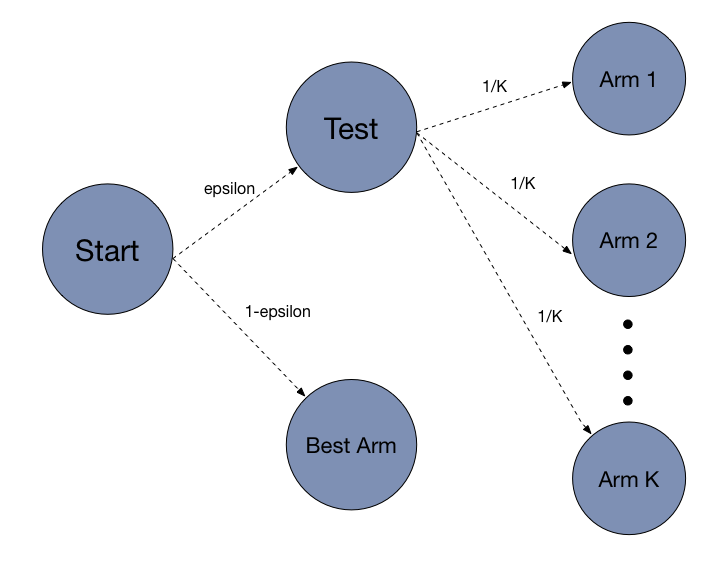
\includegraphics[scale = 0.4]{chapters/chapter02/fig02/epsilongreedy.png}}
\caption{the mechanism of epsilon-greedy}
\label{fig:epsilon}
\end{figure}

Let's be more concrete to the mechanism of $\epsilon$-greedy algorithm. It works by randomly oscillating between the purely randomized experimentation and instinct to maximize profits. The $\epsilon$-greedy is one of the easiest bandit algorithms to understand because it tries to be fair to the two opposite goals of exploration and exploitation by using a mechanism (see the Figure~\ref{fig:epsilon}). Take a simple example to understand easily: it is just like flipping a coin. If you flip a coin and it comes up heads, you should explore for a moment. But if the coin comes up tails, you should exploit.

The formal process as follows,
\begin{itemize}
\item Firstly, pick a parameter $\epsilon \in [0,1]$, 
\item Then, at each step greedily play the object with highest empirical mean reward with probability $1-\epsilon$ and play a random arm with probability $\epsilon$. 
\item Receives the reward from the arm chosen
\item Finally, update the empirical means of each arm.
\end{itemize}

%!ALGORITHM-----------------------------
%!--------------------------------------
\begin{algo}[$\epsilon$-Greedy]
%\caption{$\epsilon$-Greedy}
\label{algo:epsilon}
\begin{algorithmic}
\STATE {\ }
\STATE Initialise $P_{(\mu_1,\dots,\mu_K)}$, the prior belif of the mean payoffs of arms $1,\dots,K$. 
\FOR {each round t = 1,2,\dots, T}
	\STATE Pull arm $k_t = \begin{cases}
    \text{argmax}_{k\in \{1,\dots,K\}} P_{(\mu_k)} & \text{with probability}\ \epsilon \\
    \text{select randomly} & \text{with probability}\ 1-\epsilon
    \end{cases}$ 
    \STATE Receive reward $r_{(k_t)}$
	\STATE Update $\mu_{k_t}$ by the reward $r_{(k_t)}$.
\ENDFOR
\end{algorithmic}
\end{algo}
%!----------------------------------------

Auer~\cite{Auer02Finite} has proven that, if $\epsilon$ is allowed to be a certain function $\epsilon_t$ following the current time step $t$, namely $\epsilon_t = K/(d^2t)$, then the regret grows logarithmically like $(K \log{T}/d^2)$, provided $d$ less than the number of objects with minimum regret . While this bound has a suboptimal dependence on $d$. In Auer's~\cite{Auer02Finite} same paper, it show that this algorithm performs well in practice, but the performance degrades quickly if $d$ is not chosen as a tight lower bound.

Compared to other more complex methods, $\epsilon$-greedy is often hard to beat and reported to be often the method of the first choice as stated . In practice, however, a drawback of $\epsilon$-greedy is that it is unclear which setting of $\epsilon$ leads to good results for a given learning problem. For this reason, the experimenter has to rigorously hand tune $\epsilon$ for obtaining good results, which can be a very time-consuming task in practice depending on the complexity of the target application.

One method that aims at overcoming the above mentioned limitation of $\epsilon$-greedy is ``Value-Difference Based Exploration''(VDBE)\cite{tokic2010adaptive}. In contrast to pure $\epsilon$-greedy, VDBE adapts a state-dependent exploration-probability. The basic idea of VDBE is to extend the $\epsilon$-greedy method by controlling a state-dependent exploration probability, $\epsilon(s)$, in dependence of the value-function error instead of manual tuning. The desired behavior is to have the agent more explorative in situations when the knowledge about the environment is uncertain, i.e. at the beginning of the learning process, which is recognized as large changes in the value function. On the other hand, the exploration rate should be reduced as the agent's knowledge becomes certain about the environment, which can be recognized as very small or no changes in the value function. 